\documentclass{libs/XJTLU_format}

%\documentclass{article}

%%%%%%%%%%%%%%%%%%%%%%%%%%%%%%%%%%%%%%%%%%%%%%%%%%%%%%%%%%%%%%%%%%%%%%%%%%%%%%
% \embedvideo{<poster or text>}{<video file (MP4+H264)>}
%%%%%%%%%%%%%%%%%%%%%%%%%%%%%%%%%%%%%%%%%%%%%%%%%%%%%%%%%%%%%%%%%%%%%%%%%%%%%%
\usepackage[bigfiles]{pdfbase}
\usepackage{amssymb}
\usepackage{booktabs}
\usepackage[version=4]{mhchem}
\usepackage{siunitx}
\usepackage{pythonhighlight}

\ExplSyntaxOn
%%begin novalidate
\cs_new:Npn\embedvideo#1#2{
%%end novalidate
  \leavevmode
  \pbs_pdfobj:nnn{}{fstream}{{}{#2}}
  \pbs_pdfobj:nnn{}{dict}{
    /Type/Filespec/F~(#2)/UF~(#2)
    /EF~<</F~\pbs_pdflastobj:>>
  }
  \tl_set:Nx\video{\pbs_pdflastobj:}%
  %
  \pbs_pdfobj:nnn{}{dict}{
    /Type/RichMediaInstance/Subtype/Video
    /Asset~\video
    /Params~<</Binding/Foreground>>
  }
  %
  \pbs_pdfobj:nnn{}{dict}{
    /Type/RichMediaConfiguration/Subtype/Video
    /Instances~[\pbs_pdflastobj:]
  }
  %
  \pbs_pdfobj:nnn{}{dict}{
    /Type/RichMediaContent
    /Assets~<<
      /Names~[(#2)~\video]
    >>
    /Configurations~[\pbs_pdflastobj:]
  }
  \tl_set:Nx\rmcontent{\pbs_pdflastobj:}%
  %
  \pbs_pdfobj:nnn{}{dict}{
    /Activation~<<
      /Condition/XA
      /Presentation~<<
        /Transparent~true
        /Style/Embedded
        /PassContextClick~true
      >>
    >>
    /Deactivation~<</Condition/PC>>
  }
  %
  \hbox_set:Nn\l_tmpa_box{#1}
  \tl_set:Nx\l_box_wd_tl{\dim_use:N\box_wd:N\l_tmpa_box}
  \tl_set:Nx\l_box_ht_tl{\dim_use:N\box_ht:N\l_tmpa_box}
  \tl_set:Nx\l_box_dp_tl{\dim_use:N\box_dp:N\l_tmpa_box}
  \pbs_pdfxform:nnnnn{1}{1}{}{}{\l_tmpa_box}
  %
  \pbs_pdfannot:nnnn{\l_box_wd_tl}{\l_box_ht_tl}{\l_box_dp_tl}{
    /Subtype/RichMedia
    /BS~<</W~0/S/S>>
    /Contents~(embedded~video~file:#2)
    /NM~(rma:#2)
    /AP~<</N~\pbs_pdflastxform:>>
    /RichMediaSettings~\pbs_pdflastobj:
    /RichMediaContent~\rmcontent
  }
  \phantom{#1}
}%
\ExplSyntaxOff
%%%%%%%%%%%%%%%%%%%%%%%%%%%%%%%%%%%%%%%%%%%%%%%%%%%%%%%%%%%%%%%%%%%%%%%%%%%%%%


% % Inserting the preamble file with the packages
% %%%%%%%%%%%%%%%%%%%%%%%%%%%%%%%%%%%%%%%%%%%%%%%%%%%%%%%%%%%%%%%%%%%%%
%% This file contains the packages that can be used in the beamer. %%
%%%%%%%%%%%%%%%%%%%%%%%%%%%%%%%%%%%%%%%%%%%%%%%%%%%%%%%%%%%%%%%%%%%%%
% Package to fonts family
\usepackage[T1]{fontenc}
% Package to accentuation
\usepackage[utf8]{inputenc}
% Package to Figures
\usepackage{graphicx}
% Package to the colors
\usepackage{color}
% Package to the colors
\usepackage{xcolor}
% Packages to math symbols and expressions
\usepackage{amsfonts, amssymb, amsmath}
% Package to multiple lines and columns in table
\usepackage{multirow, array} 
% Package to create pseudo-code
% For more detail of this package: http://linorg.usp.br/CTAN/macros/latex/contrib/algorithm2e/doc/algorithm2e.pdf
\usepackage{algorithm2e}
% Package to insert code
\usepackage{listings} 
\usepackage{keyval}
% Package to justify text
\usepackage[document]{ragged2e}
% Package to manage the bibliography
\usepackage[backend=biber, style=numeric, sorting=none]{biblatex}
% Package to facilities quotations
\usepackage{csquotes}
% Package to use multicols
\usepackage{multicol}
\usepackage{transparent}

% % Inserting the references file
% \bibliography{references.bib}

% % Title
% \title[MAT 214_Processing and Properties of Ceramic Materials]{\textbf{MAT 214: Processing and Properties of Ceramic Materials}}
% % Subtitle
% \subtitle{Introduction to Ceramic Materials}
% % Author of the presentation
% \author{Prof. Joshua C. Agar}
% % Institute's Name
% \institute[Lehigh University]{
%     % email for contact
%     \normalsize{\email{jca318@lehigh.edu}}
%     \newline
%     % Department Name
%     \department{Materials Science and Engineering}
%     \newline
%     % University name
%     \university{Lehigh Univeristy}
% }
% % date of the presentation
% \date{\today}

% %\newcommand*{\keys}{\fontfamily{cmtt}\selectfont}

%%%%%%%%%%%%%%%%%%%%%%%%%%%%%%%%%%%%%%%%%%%%%%%%%%%%%%%%%%%%%%%%%%%%%%%%%%%%%%


% Inserting the preamble file with the packages
%%%%%%%%%%%%%%%%%%%%%%%%%%%%%%%%%%%%%%%%%%%%%%%%%%%%%%%%%%%%%%%%%%%%%
%% This file contains the packages that can be used in the beamer. %%
%%%%%%%%%%%%%%%%%%%%%%%%%%%%%%%%%%%%%%%%%%%%%%%%%%%%%%%%%%%%%%%%%%%%%
% Package to fonts family
\usepackage[T1]{fontenc}
% Package to accentuation
\usepackage[utf8]{inputenc}
% Package to Figures
\usepackage{graphicx}
% Package to the colors
\usepackage{color}
% Package to the colors
\usepackage{xcolor}
% Packages to math symbols and expressions
\usepackage{amsfonts, amssymb, amsmath}
% Package to multiple lines and columns in table
\usepackage{multirow, array} 
% Package to create pseudo-code
% For more detail of this package: http://linorg.usp.br/CTAN/macros/latex/contrib/algorithm2e/doc/algorithm2e.pdf
\usepackage{algorithm2e}
% Package to insert code
\usepackage{listings} 
\usepackage{keyval}
% Package to justify text
\usepackage[document]{ragged2e}
% Package to manage the bibliography
\usepackage[backend=biber, style=numeric, sorting=none]{biblatex}
% Package to facilities quotations
\usepackage{csquotes}
% Package to use multicols
\usepackage{multicol}
\usepackage{transparent}

% Inserting the references file
\bibliography{references.bib}

% Title
\title[MAT 214 Spring 2022]{\textbf{MAT 214: Processing and Properties of Ceramic Materials}}
% Subtitle
\subtitle{Point Defects and Charge}
% Author of the presentation
\author{Prof. Joshua C. Agar}
% Institute's Name
\institute[Lehigh University]{
    % email for contact
    \normalsize{\email{jca318@lehigh.edu}}
    \newline
    % Department Name
    \department{Materials Science and Engineering}
    \newline
    % University name
    \university{Lehigh Univeristy}
}
% date of the presentation
\date{\today}

%%%%%%%%%%%%%%%%%%%%%%%%%%%%%%%%%%%%%%%%%%%%%%%%%%%%%%%%%%%%%%%%%%%%%%%%%%%%%%%%%%
%% Start Document of the Presentation                                           %%               
%%%%%%%%%%%%%%%%%%%%%%%%%%%%%%%%%%%%%%%%%%%%%%%%%%%%%%%%%%%%%%%%%%%%%%%%%%%%%%%%%%
\begin{document}

% insert the code style
%%%%%%%%%%%%%%%%%%%%%%%%%%%%%%%%%%%%%%%%%%%%%%%%%%%%%%%%%%%%%%%%%%%%%%%%%%%%%%%%%%%
%% This file contains the style of the codes show in slides.                     %%
%% The package used is listings, but it possible to used others.                 %%
%%%%%%%%%%%%%%%%%%%%%%%%%%%%%%%%%%%%%%%%%%%%%%%%%%%%%%%%%%%%%%%%%%%%%%%%%%%%%%%%%%%

% color used in the code style
\definecolor{codegreen}{rgb}{0,0.6,0}
\definecolor{codegray}{rgb}{0.5,0.5,0.5}
\definecolor{codepurple}{rgb}{0.58,0,0.82}
\definecolor{codebackground}{rgb}{0.95,0.95,0.92}

% style of the code!
\lstdefinestyle{codestyle}{
    backgroundcolor=\color{codebackground},   
    commentstyle=\color{codegreen},
    keywordstyle=\color{magenta},
    numberstyle=\tiny\color{codegray},
    stringstyle=\color{codepurple},
    basicstyle=\ttfamily\footnotesize,
    frame=single,
    breakatwhitespace=false,         
    breaklines=true,                 
    captionpos=b,                    
    keepspaces=true,                 
    numbers=left,                    
    numbersep=5pt,                  
    showspaces=false,                
    showstringspaces=false,
    showtabs=false,                  
    tabsize=2,
    title=\lstname 
}

\lstset{style=codestyle}


%% ---------------------------------------------------------------------------
% First frame (with tile, subtitle, ...)
\begin{frame}{}
    \maketitle
\end{frame}

\section{Learning Objectives:}
\begin{frame}{Learning Objectives}
\begin{itemize}
    \item A knowledge of the types of defects that can form in ceramic materials
    \pause
    \item A working knowledge of Kröger-Vink notation and conservation laws
    \pause
    \item Thermodynamics of defect formation
    \pause
    \item Understanding of the Law of Mass Action
    \pause
    \item How to calculate the temperature dependence of defect concentration
    \pause
    \item An understanding of common defect reactions Schottky, Frenkel, Electronic, and non-stoichiometry
\end{itemize}
    
\end{frame}

\section{Ceramic Defects}
\begin{frame}{Are Defects Different in Ceramics?}
    \begin{itemize}
        \item<1-> Real crystals contain a variety of imperfections or defects
        \item<2-> In crystals and ceramic glasses the structure and chemistry are determined by defect mobility
    \end{itemize} \\[0.3cm]
    
    \pause
    Key Differences:\\[0.3cm]
    \begin{itemize}
        \item<3-> The concentration of impurities in ceramics is usually much greater than that of intrinsic defects
        \item<4-> Dislocations are much less important for deformation mechanisms
        \item<5-> Surfaces and interfaces are extremely important
        \item<6-> Pores and voids are much more important in determining properties
    \end{itemize}
\end{frame}

\begin{frame}{Vacancies}
An atom that is not present on a site that it should be\\[0.3cm]\pause

\emph{Schottky Defect:} is a set of vacancies created by removing one atom for each atom in the chemical formula.\\[0.3cm]

\centering
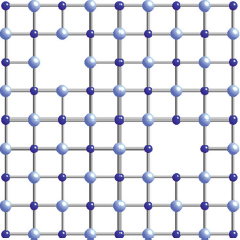
\includegraphics[height=1in]{Silde_Template/Images/Schottkey.png} \\[0.3cm] \pause

\justifying
\textbf{Example:} In a stoichiometric crystal such as MgO, we get a pair of vacancies, one on the Mg sublattice and one on the O sublattice
    
\end{frame}
    
\begin{frame}{Interstitials}
If an atom is present on any site that would be unoccupied in a perfect crystal, then that atom is an interstitial \\[0.3cm]\pause

\centering
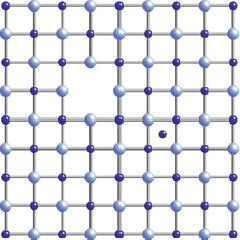
\includegraphics[height=1in]{Silde_Template/Images/Intersitial.png} \\[0.3cm] \pause

\justifying
\emph{Frenkel Defect:} is a vacancy + interstitial pair formed by removing an atom from its site in the crystal structure and putting it into an interstice\\[0.3cm]

\pause
\justifying
Frenkel defects are the underlying mechanisms for old-school photography
    
\end{frame}

\begin{frame}{Misplaced atoms}

If an atom is present on a crystal site that should be occupied by a different atom, \pause that atom is a misplaced atom and may be called an antisite defect. \\[0.3cm]\pause

\centering
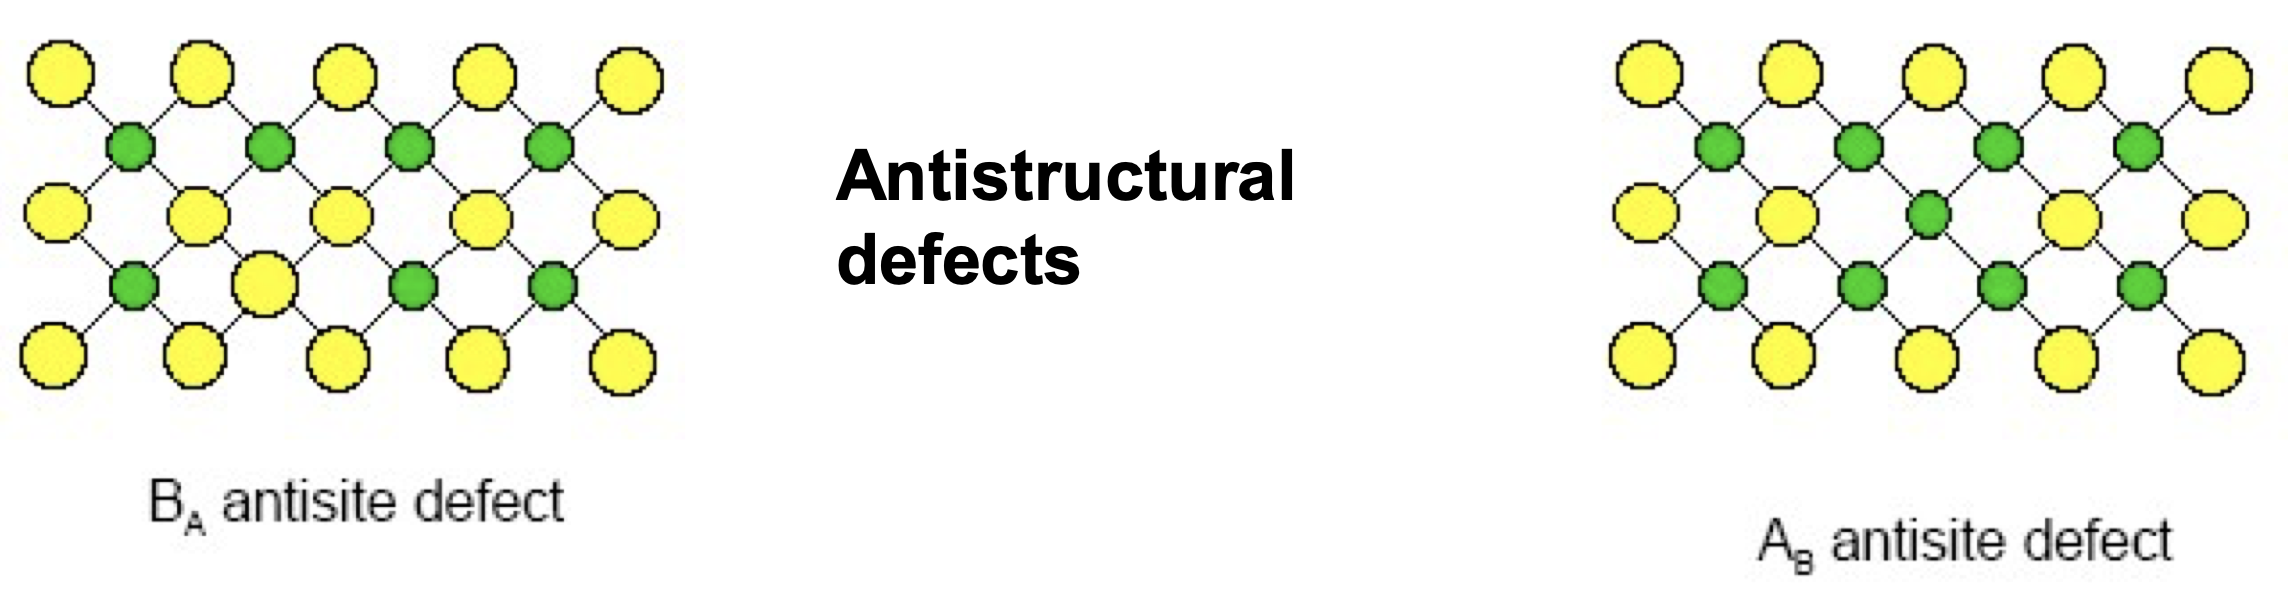
\includegraphics[height=1in]{Silde_Template/Images/Antisite_defect.png} \\[0.3cm] \pause

\begin{itemize}
    \item Antisite defects common in systems with covalent bonds \pause
    \item Can happen in ionic bonded materials but it is not possible for cations and anions to switch places
\end{itemize}

\end{frame}

\begin{frame}{Associated Centers}
    When two point defects interact so they can be considered a single defect, they are called an associated center or, if more atoms are involved, a defect cluster or a defect complex \pause
    
    \begin{itemize}
        \item Most of these give rise to color centers $\rightarrow$ gives rise to color in crystals \pause
        \item Electron or hole trapped in a vacancy center
    \end{itemize}
    
    \centering
    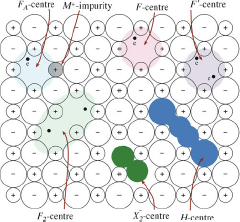
\includegraphics[height=1.5 in]{Silde_Template/Images/Color_center.png} \\[0.3cm]
\end{frame}

\begin{frame}{Solute (substitutional) atoms}
It is possible to substitute atoms in ionic and covalent solids without changing the crystal structure\\[0.3cm] \pause

\begin{itemize}
    \item Cu alloys, we can add up to 30 at.\% Zn before the structure is changed \pause
    \item Substitute Ge in Si, but the solubility is limited due to the difference in atomic size \pause
    \item In GaAs, we can replace the Ga atom by Al on the group III sublattice, giving a complete solid solution \ce{GaAl_{1-x}As_x}
\end{itemize}
    
\end{frame}

\begin{frame}{Electronic Defects}
    Electrons and holes can both exist in ceramics. \pause
    
    \begin{itemize}
        \item They may be associated with particular ions, in which case they are simply charged point defects \pause
        \item Kröger-Vink notation to identify these different point defects \pause
        \item We need such a notation because of one of the most special features about ceramics — the charge
    \end{itemize}
    
\end{frame}

\begin{frame}{Why are Defects Special in Ceramics? -- Revisiting}
\begin{itemize}
    \item Vacancies, interstitials, and substitutional defects can all be charged \pause
    \begin{itemize}
        \item The special point defect in ceramics is the charged vacancy
        \item Frenkel and Schottky defects are overall neutral \pause
    \end{itemize}
    \item Association of defects is particularly important for ceramics because Coulombic interactions are both strong and long range \pause
    \item Electronic structure is increasingly important as it can influence band gaps and conductivity \pause
    \item Nonstoichiometry is important because the concentration of point defects can be very large
\end{itemize}
    
\end{frame}

\section{Formulations of Defects}
\begin{frame}{Conservation Laws}
\begin{enumerate}
    \item We must conserve mass
    \begin{itemize}
        \item Defect reactions cannot result in the loss of atoms \pause
    \end{itemize}
    \item We must preserve number the nature of the structure
    \begin{itemize}
        \item This means that if lattice sites are added they need to be equivalent to one formula unit of the structure \pause
    \end{itemize}
    \item Charge must be balanced
    \begin{itemize}
        \item If a charge defect is added it must be offset by an equal and opposite charged defect to maintain neutrality
    \end{itemize}
\end{enumerate}
    
\end{frame}

\begin{frame}{Kröger-Vink Notation}
\\
We can describe chemical expressions involving defects using Kröger-Vink Notation
\pause

\begin{itemize}
    \item Main symbol - Defect species as an element or vacancy \pause
    \item Subscript - Element site or interstitial site \pause
    \item Superscript - Effective charge ($\bullet$ positive, $'$ negative) \pause
\end{itemize}\\[0.3cm]

Examples:
\begin{center}
\begin{tabular}{l c}
 Oxygen Vacancy & 
 \ce{V_o^{$\bullet\bullet$}} \\ \pause 
 Magnesium vacancy & 
 \ce{V_{Mg}^{$''$}} \\ \pause
 Magnesium on magnesium site & 
 \ce{Mg_{Mg}^{$x$}} \\ \pause 
 Oxygen interstitial & \ce{O_{i}^{$''$}} \\  \pause
 Magnesium interstitial & \ce{Mg_{i}^{$\bullet\bullet$}}  \\ \pause 
 Aluminum on magnesium site & \ce{Al_{Mg}^{$\bullet$}} \\ \pause
 Sodium on magnesium site & \ce{Na_{Mg}^{$'$}} \\ \pause 
 Nickel on magnesium site & \ce{Ni_{Mg}^{$x$}} \\ \pause
 Nitrogen on oxygen site & \ce{N_{O}^{$'$}}
\end{tabular}
\end{center}

\end{frame}

\begin{frame}{Equilibrium Defect Concentration}
It is important to have a sense of how many defects are present in thermal equilibrium\\[0.3cm] \pause

At a given temperature the number of vacancy is defined by the Gibb's Free Energy: \\[0.1cm] \pause

\centering
$\Delta G = \Delta H - T \Delta S  $\\[0.1cm] \pause
\justifying
G is gibbs free energy, H is the enthalpy, T is the temperature, and S is the entropy.

\pause
\centering
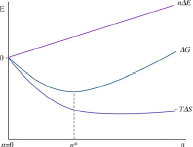
\includegraphics[height=1in]{Silde_Template/Images/Defect_formation.png}
\\
\justifying
This means that at any temperature above T = 0 there will be some defects. 

\end{frame}

\begin{frame}{Law of Mass Action}
\begin{itemize}
    \item The rate of a chemical reaction is proportional to the activity or concentration of the reactive species
\end{itemize}\\[6 pt]

\pause
For example, consider the reaction: \\[3 pt]

\ce{\emph{a}A + \emph{b}B -> \emph{c}C + \emph{d}D}\\[6 pt]

\pause
The Law of Mass Action states that the equilibrium reaction constant is: \\[3 pt]

\centering
$K_{eq} = \frac{[C]^c[D]^d}{[A]^a[B]^b}$
    
\end{frame}

\section{Schottky}
\begin{frame}{Schottky Defect Equations:}
Equation for a Schottky Defect: \\[0.1cm]
\centering
$null = V_{Mg}^{''} + V_{O}^{\bullet \bullet}$\\[0.3cm] \pause

\justifying
For dilute solutions, the Law of Mass Action Implies:\\[0.1cm]
\centering
$K_s = [V_{Mg}^{''}][V_{O}^{\bullet \bullet}]$ \pause $= \exp(\frac{-\Detla G_s}{kT})$ \pause $= \exp(\frac{\Detla S_s}{kT}) \exp(\frac{-\Detla H}{kT})$\\[0.1cm]

\justifying
Where $\Delta$G is gibbs free energy, $\Delta$H is the enthalpy, T is the temperature, and $\Delta$S is the entropy.\\[0.3cm] \pause

\justifying
If you assume that Schottky are the only source of defects:

\centering
$[V_{Mg}^{''}] = [V_{O}^{\bullet \bullet}] = K_s^{1/2} = \exp(\frac{-\Detla G_s}{2kT}) = \exp(\frac{\Detla S_s}{2kT})\exp(\frac{-\Detla H}{2kT})$
    
\end{frame}

\begin{frame}{Example Problem}
\simplebox{Consider \ce{NaCl} where defects are governed by schottky defects. \\ Write the defect reaction. \\ Determine the number of defects at 800$^\circ$C assuming $\Delta H$ = 236 kJ/mol and $\Delta S = \num{1.28e-22} J / atom K$. \\ Compare the number of defects to \ce{MgO} assuming $\Detla H = 670 kJ/mol$. You can assume the entropy of a schottky defect is the same as NaCl since they have the same crystal structures.} \pause

In NaCl at 800$^\circ$:
\emph{It is most simple to work in eV}:\\
\centering
$\Delta H = 2.45 eV/atom = 236 kJ/mol$ \pause

\centering
$e^{-\Delta H_s/2kT} = e^{\frac{-2.45 eV\,atom}{2 (\num{8.617e-5} eV/ atom\,K)(800 + 273 K)}} = \num{1.76e-6}$
$e^{\Delta S / 2 k} = e^{\frac{\num{1.28e-22} J/ atom\,K}{2 (\num{1.38e-23} J/atom\,K})} = 103.3$ \pause
 
$[defects] = \exp(\frac{\Detla S_s}{2kT})\exp(\frac{-\Detla H}{2kT}) = \num{1.76e-6} \times 103.3 = \num{1.82e-3}$ or 182 ppm\\[6 pt]

\pause
\justifying
This is significant enough to control properties but requires high temperature

\end{frame}

\begin{frame}{Example Problem}
\simplebox{Consider \ce{NaCl} where defects are governed by schottky defects. \\ Write the defect reaction. \\ Determine the number of defects at 800$^\circ$C assuming $\Delta H$ = 236 kJ/mol and $\Delta S = \num{1.28e-22} J / atom K$. \\ Compare the number of defects to \ce{MgO} assuming $\Detla H = 670 kJ/mol$. You can assume the entropy of a schottky defect is the same as NaCl since they have the same crystal structures.}

\justifying
For MgO $\Delta H_{MgO} = 7 eV$, thus the defect density is:

\centering
$e^{-\Delta H_s/2kT} = e^{\frac{-7 eV\,atom}{2 (\num{8.617e-5} eV/ atom\,K)(800 + 273 K)}} = \num{3.63e-17}$
$[defects] = \exp(\frac{\Detla S_s}{2kT})\exp(\frac{-\Detla H}{2kT}) = \num{(3.63e-17)} 103.3 = \num{3.75e-15}$\\[0.3cm] \pause

\justifying
This is 11 orders of magnitude less because of the stronger bonding energy!

\end{frame}
 
\begin{frame}{Putting this in Context}

With the exception of Si wafers ceramics generally have impurities on the order of 0.1\% or higher \pause $\rightarrow$ Thus intrinsic defects are rarely of significance. The properties are dominated by impurities or dopants. This is called \textbf{extrinsic}\\[0.3cm] \pause

\emph{Important Definitions:}\\[6 pt]
\textbf{Intrinsic Properties:} Properties of a material that result from the pure material at thermal equilibrium\\\pause
\textbf{Extrinsic Properties:} Properties of a material that result from deviations from perfect stoichiometry 
    
\end{frame}
\section{Frenkel}
\begin{frame}{Frenkel Defects}

Frenkel Defects are vacancy-interstitial pairs. Considering \ce{MgO} the equation for a Frenkel Defect:\\[0.1cm] \pause

\centering
$Mg_{Mg}^x=V_{Mg}^{''} + Mg_{i}^{\bullet \bullet}$\\[0.1cm] \pause

\justifying
For dilute solutions the cation Law of Mass Action implies:

\centering
$[V_{Mg}^{''}][Mg_{i}^{\bullet \bullet}] = K_F = \exp(\frac{-\Detla G_s}{kT}) = \exp(\frac{\Detla S_s}{kT})\exp(\frac{-\Detla H}{kT})$ \\[6 pt] \pause

\justifying
The anion expression can be written as: 

\centering
$[V_{O}^{\bullet \bullet}][O_{i}^{''}] = K_F = \exp(\frac{-\Detla G_s}{kT}) = \exp(\frac{\Detla S_s}{kT})\exp(\frac{-\Detla H}{kT})$ \\[6 pt] \pause

\justifying
The enthalpy of Frenkel defect formation is highly-dependent on the crystal structure
\begin{itemize}
    \item Frenkel defects are preferred when the crystal structure is open with large interstitial sites. \pause
    \item \ce{NaCl} is fairly closed packed Schottky defects preferred.
    \item \ce{CaF2}, F sits at the FCC lattice and thus can easily fit into the octahedral sites. 
\end{itemize}
\end{frame}

\section{Electronic}
\begin{frame}{Electronic Defects}
Electronic defects associated with electronic excitation of energy greater than the band gap:\\[0.1cm]

\centering
$null = e^{'} + h^{\bullet}$\\[6 pt]
\pause

\justifying
Using the law of mass action:\\[0.1cm]

\centering
$np = K_{elec} = N_c N_v \exp{(-E_g/kT)}$

\justifying
Where n - is the number of electron carriers, p - is the number of hole carriers, $N_c$ - is the density of states in the conduction band, $N_v$ is the density of states in the valence band, and $E_g$ is the band gap.\\[0.1cm]
\pause

If the carriers are intrinsic (not from defects), $n=p$:\\[6 pt]
\centering
$n=p=(N_c N_v)^{1/2}\exp{(-E_g/2kT)}$

\end{frame}

\begin{frame}{Example NaCl:}

\centering
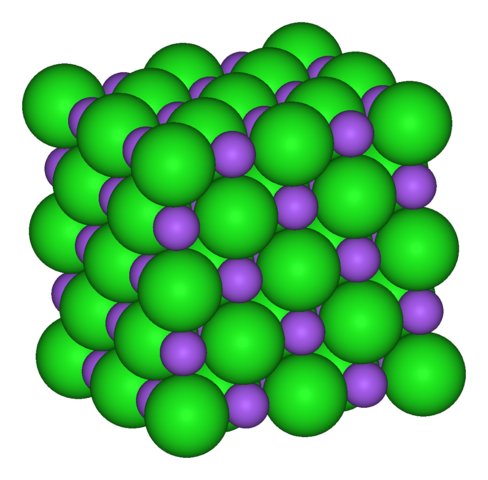
\includegraphics[height=1in]{Silde_Template/Images/Sodium-chloride-3D-vdW.png} \\[0.3cm] \pause

\begin{itemize}
    \item Valence band Cl 3p state are all filled at 0K 
    \item Conduction band Na 3s states are normally empty \pause
    \item Forming an electronic defect requires taking an electron away from $Cl^{\bullet}$ ion giving it to $Na^{+}$ ion $\rightarrow$ This is highly unfavorable $E_g \approx 8-10 eV$ \pause
    \item Compounds with transition metals (e.g., Ti, Mn, etc.) have multiple oxidation states band gap between 3-4 eV $\rightarrow$ much more favorable to have electronic defects
\end{itemize}
    
\end{frame}

\begin{frame}{Acceptor Defects:}

\begin{itemize}
    \item Acceptors have a lower valence than the atom they replace $\rightarrow$ They have a negative effective charge \pause
    \item Remember acceptors accept an electron \pause
    \item Law of mass action cannot be used because we have impurities being incorporated into the reaction \pause
\end{itemize}\\[0.3cm]

Example \ce{Na2O} in \ce{MgO}:

\centering
\ce{Na2O ->[2MgO] 2Na_{Mg}^' + O_O^x + V_O^{$\bullet \bullet$}}\\[6 pt]

\justifying
Charge neutrality approximation condition:\\
\centering
\ce{[Na_{Mg}^'] = 2[V_O^{$\bullet \bullet$}]}

\end{frame}


\begin{frame}{Acceptor Defects:}

\begin{itemize}
    \item Acceptors have a lower valence than the atom they replace $\rightarrow$ They have a negative effective charge
    \item Remember acceptors accept an electron
    \item Law of mass action cannot be used because we have impurities being incorporated into the reaction
\end{itemize}\\[0.3cm]

Example 2 \ce{NiO} in \ce{Al2O3}:

\centering
\ce{3NiO ->[Al2O3] 3Ni_{Al}^' + 2O_O^x + V_O^{$\bullet \bullet$}}\\[0.1cm]
or\\
\ce{3NiO ->[Al2O3] 2Ni_{Al}^' + 3O_O^x + Ni_i^{$\bullet \bullet$}}\\[6 pt] \pause

\justifying
Charge neutrality approximation condition:\\

\centering
\ce{[Ni_{Al}^'] = 2[V_O^{$\bullet \bullet$}]}
or
\ce{[Ni_Al^'] = 2[Ni_i^{$\bullet \bullet$}]}\\[6 pt] \pause

\justifying
It is not clear which mechanism will take place, it depends on energetic. In \ce{Al2O3} 1/3 of the octahedral sites are free thus occupation is a real possibility. 

\end{frame}

\begin{frame}{Donor Defects:}
\begin{itemize}
    \item Donor impurities have a higher valence than the host ions they replace $\rightarrow$ They have an effective positive charge \pause
    \item Remember Donors donate an electron \pause
    \item Law of mass action cannot be used because we have impurities being incorporated into the reaction
\end{itemize}

\pause
Example \ce{CaCl2} in NaCl:\\[0.1cm]

\centering
\ce{CaCl2 ->[2NaCl] Ca_Na^{$\bullet$} + 2Cl_Cl^x + V_Na^{'}}\\[6 pt] \pause

\justifying
Charge neutrality approximation condition: \\[0.1cm]

\centering
[\ce{Ca_{Na}^{$\bullet$}}] = [\ce{V_{Na}^'}]

\end{frame}

\begin{frame}{Donor Defects:}

Example 2 \ce{Nb2O5} in \ce{BaTiO3}:\\[0.1cm]

\pause
\centering
\ce{Nb2O5 ->[2BaTiO3] 2Nb_{Ti}^{$\bullet$} + 5O_O^x + 1/2O2(g) +  2e^{'}}\\[0.1cm]

\pause
\justifying
Charge neutrality approximation condition: \\[0.1cm]

\centering
[\ce{Nb_{Ti}^{$\bullet$}}] = [\ce{e^'}]

\pause
\justifying
At high concentrations of Nb mechanism changes

\centering
\ce{2Nb2O5 ->[4BaTiO3] 4Nb_{Ti}^{$\bullet$} + V_{Ti}^{''''} + 10O_O}\\[6 pt]

\pause
\justifying
Nb-Doped \ce{BaTiO3} goes from blue and semiconducting at low defects to white and insulating at higher concentrations due to the nature of the defect.

\end{frame}

\section{Nonstoichiometry}
\begin{frame}{Oxidation Reactions}
Many ceramics are oxides they can react to changing oxygen environments\\[0.1cm] \pause

Oxidation reactions involve a atom giving up an electron to increase its oxidation state (higher + charge) $\rightarrow$ most commonly this is with oxygen but it does not have to be.\\ [6 pt]

\pause
Oxidation Reaction:\\

\centering
\ce{1/2O2(g) <=> O_O^x + V_M^{''} + 2h^{$\bullet$}}\\[0.1cm] \pause

\justifying
Using the law of mass action:

\centering
$K_ox = \frac{p^2 V_m^{''}}{P_{O_2}^{1/2}}$\\[0.1cm] \pause

\justifying
This reaction can be faster in the presence of transition metals:\\[2 pt]

\centering
\ce{Fe^{2+} -> Fe^{3+} = Fe_{Fe}^{$\bullet$} = h^{$\bullet$}}\\[6 pt]
\pause

\justifying
\ce{FeO}, \ce{CoO} and \ce{NiO} can accommodate a significant amount of nonstoichiometry \ce{Fe_{(1-x)}O}, \ce{Ni_{(1-x)}O} and \ce{Co_{(1-x)}O}, where x is in the range of 0.01 - 0.15, whereas \ce{MgO} and \ce{Al2O3} can not.
    
\end{frame}

\begin{frame}{Reduction Reactions}

Reduction reactions involve a atom gaining an electron to decrease its oxidation state (lower + charge)

\pause
Reduction Reaction:\\[3pt]

\centering
\ce{O_o^x -> V_O^{$\bullet \bullet$} + 1/2O_2(g) + 2e^{'}}\\[6 pt] \pause

\justifying
Using the law of mass action:

\centering
$K_{red} = n^2 V_O^{$\bullet \bullet$} P_{O_2}^{1/2}$ \\[6 pt] \pause

\justifying
Reduction reactions are favorable when there are reducible species present \pause $\rightarrow$ $Ti^{4+}$ can reduce to $Ti^{3+}$\\[3 pt]

\centering
\ce{Ti^{3+} = Ti_{Ti}^{'}}

\end{frame}

\section{Concepts to Master}
\begin{frame}{Concepts to Master}
\begin{itemize}
    \item Names and occupancy for common types of defects \pause
    \item Working knowledge of the Law of Mass Action \pause
    \item Working knowledge of how to write defect reactions using Kröger-Vink notation \pause
    \item Understanding of thermodynamic expression for defect reactions \pause
    \item Understanding of dopant defects \pause
    \item Working knowledge of expressions for oxidation and reduction reactions
\end{itemize}
\end{frame}
% \begin{frame}{Metals}

% \begin{itemize}
%     \item Constructed of atoms held together by delocalized electrons
%     \pause
%     \item They are commonly found as alloys with metallic and non-metallic elements
%     \pause
%     \item Delocalized electrons give metallic properties (e.g., good thermal and electrical conductivity)
%     \pause
%     \item Metallic bonding allows for closed-packed crystal structures that permit plastic deformation
% \end{itemize}
    
% \end{frame}

% \begin{frame}{Polymers}
% \begin{itemize}
%     \item Macromolecules formed by covalent bonding of many simpler molecular units called mers 
%     \pause
%     \item Most polymers are organic compounds based on carbon, hydrogen, and other nonmetals such as sulfur and chlorine 
%     \pause
%     \item The bonding between the molecular chains determines many of their properties
%     \pause
%     \item Many of the plastics that we are familiar with are actually combinations of polymers and often include fillers and other additives to give the desired properties and appearance
% \end{itemize}
% \end{frame}

% \begin{frame}{Ceramics}
% What are ceramics? 
% \pause
% \vspace{1em}

% \begin{itemize}
%     \item “mixed” bonding a combination of covalent, ionic, and sometimes metallic
%     \pause
%     \item They consist of arrays of interconnected atoms; there are no discrete molecules
%     \item The majority of ceramics are compounds of metals or metalloids and nonmetals
%     \pause
%     \item Most frequently they are oxides, nitrides, and carbides, however, diamond and graphite are considered ceramics.
% \end{itemize}
% \pause

% \vspace{1em}
% \textbf{Most solid materials that are not metal, plastic, or derived from plants or animals are ceramics}

% \end{frame}

% \begin{frame}{Semiconductors}

% \begin{itemize}
%     \item Only class of material based on a property
%     \pause
%     \item They are usually defined as having electrical conductivity between that of a good conductor and an insulator
%     \pause
%     \item The conductivity is strongly dependent upon the presence of small amounts of impurities
%     \pause
%     \item Classically, semiconductors have been limited to materials with a band gap $<3eV$, but there is growing commercial interest in large band gap semiconductors for high-temperature electronics.
% \end{itemize}
    
% \end{frame}

% \begin{frame}{Composites}
%     \begin{itemize}
%         \item Composites are materials formed by more than one material (sometimes this is extended to phase)
%         \pause
%         \item Usually there is a matrix and a filler
%         \pause
%         \item it is quite common to have ceramic composites
%     \end{itemize}
%         \pause
%         \centering
%         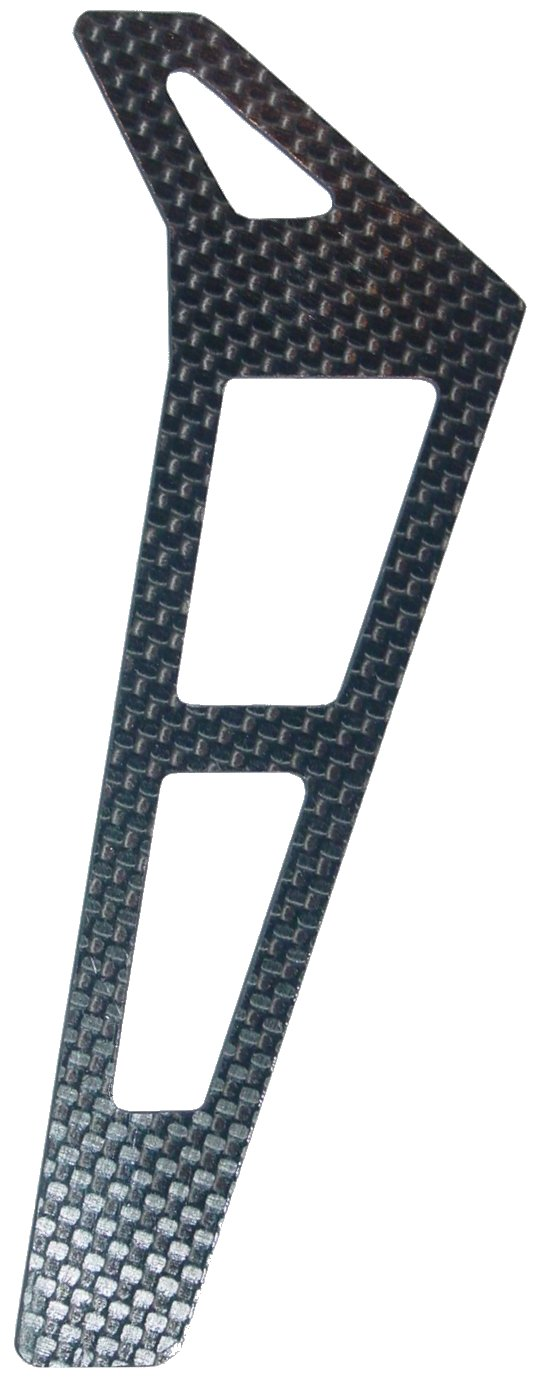
\includegraphics[height=1in]{Silde_Template/images/carbon_fiber.jpeg}
    
    
% \end{frame}

% \begin{frame}{Ceramic Ontologies and Exceptions}
% Exclusionary definition: Ceramic materials are inorganic, non-metallic solids.
% \pause

% \begin{itemize}
%     \item All inorganic semiconductors are ceramics
%     \pause
%     \item A materials ceases to be a ceramic when melted
%     \pause
%     \item All high-temperature superconductors are ceramics
%     \pause
%     \item Ice even though it is an inorganic material in the solid phase is not a ceramic
%     \pause
%     \item Glasses live in a gray area - it is really a supercooled liquid
% \end{itemize}
    
% \end{frame}

% \begin{frame}{Ceramic Ontologies and Exceptions}
% Ceramics cannot be defined based on their properties

% \begin{itemize}
%     \item We can’t say “ceramics are brittle” because some can be superplastically deformed and some metals can be more brittle: a rubber hose or banana at 77 K shatters under a hammer
%     \pause
%     \item We can’t say “ceramics are insulators” unless we put a value on the band gap (Eg) where a material is not a semiconductor.
%     \pause
%     \item We can’t say “ceramics are poor conductors of heat” because diamond has the highest thermal conductivity of any known material. Porous ceramics have some of the lowest thermal conductivity of any known materials.
% \end{itemize}
    
% \end{frame}

% \section{Properties of Ceramics}

% \begin{frame}{Brittleness}
%     \centering
%     
\includegraphics[height=1in]{Silde_Template/images/plate.jpeg}
    
%     \begin{itemize}
%         \item This property is recognized from personal experience, such as dropping a glass beaker or a dinner plate
%         \pause
%         \item The reason that the majority of ceramics are brittle is the mixed ionic-covalent bonding that holds the constituent atoms together
%         \pause
%         \item most ceramics are brittle at room temperature but not necessarily at elevated temperatures -- they can become viscous
%     \end{itemize}
    
% \end{frame}

% \begin{frame}{Poor electrical and thermal conduction}
    
%     \begin{itemize}
%         \item The valence electrons are tied up in bonds and are not free as they are in metals
%         \pause
%         \item Diamond, which we classified as a ceramic, has the highest thermal conductivity of any known material. \pause The conduction mechanism is due to phonons, not electrons.
%         \pause
%         \item The oxide ceramic $ReO_{3}$ has an electrical conductivity at room temperature similar to that of Cu
%         \pause
%         \item The mixed oxide $YBa_{2}Cu_{3}O_{7}$ is an HTSC; it has zero resistivity below 92 K
%     \end{itemize}
    
% \end{frame}

% \begin{frame}{Compressive Strength}
%     \centering
%     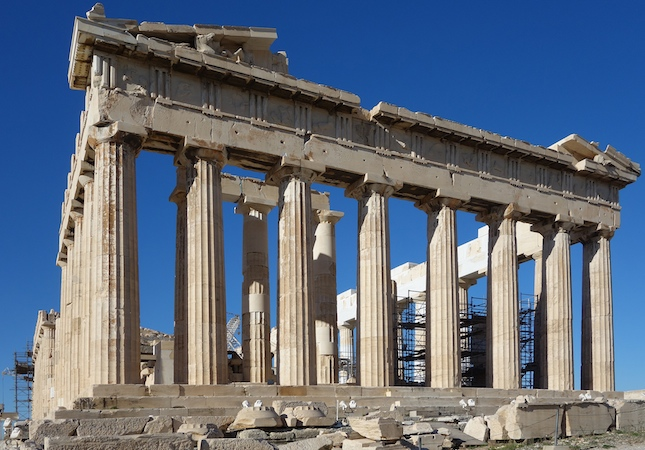
\includegraphics[height=1in]{Silde_Template/images/Greekcolumns.jpeg}
    
%     \begin{itemize}
%         \item Ceramics are stronger in compression than in tension, whereas metals have comparable tensile and compressive strengths \pause
%         \item This difference is important when we use ceramic components for load-bearing applications \pause
%         \item Ceramics generally have a low degree of toughness, although combining them in composites can dramatically improve this property
%     \end{itemize}
% \end{frame}

% \begin{frame}{Chemical insensitivity}

% \centering
% 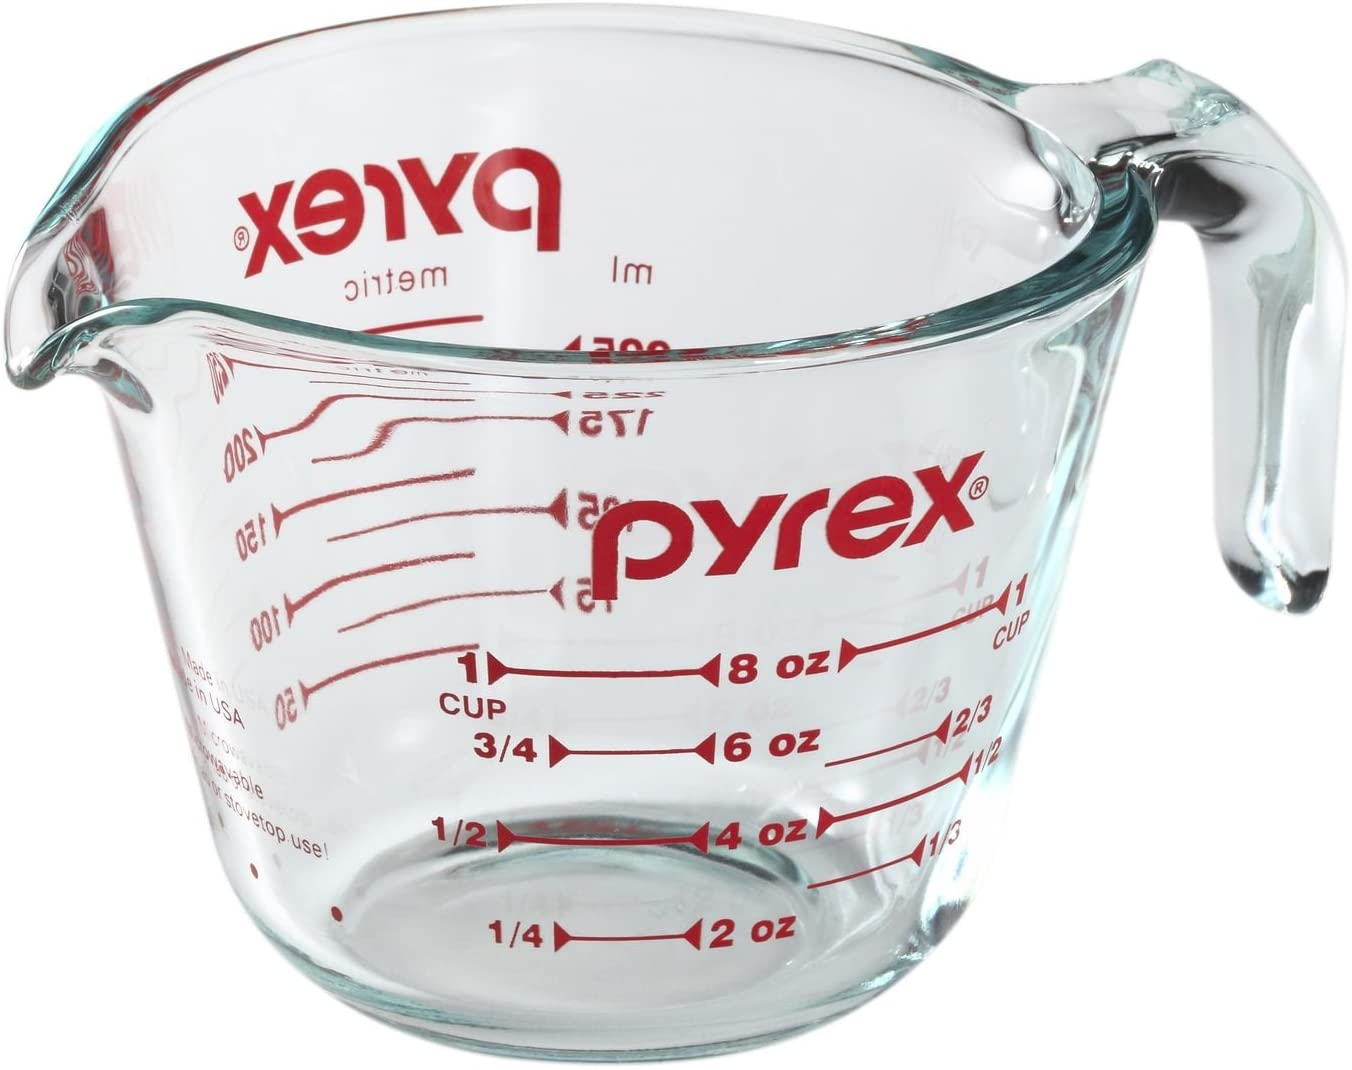
\includegraphics[height=1in]{Silde_Template/images/pyrex.jpg}

% \begin{itemize}
%     \item A large number of ceramics are stable in both harsh chemical and thermal environments
%     \pause
%     \item Example Pyrex: resistant to many corrosive chemicals, \pause stable at high temperatures (does not soften until 1,100 K),\pause and resistant to thermal shock because of its low coefficient of thermal expansion ($33x10^{-7} K^{-1}$)
% \end{itemize}
    
% \end{frame}

% \begin{frame}{Transparent}

% \centering
% 
\includegraphics[height=1in]{Silde_Template/images/apple-watch-series-7-lte-45mm-silver-stainless-steel-silver-milanese-loop-mkje3ll-a-sku4790177.jpeg}

% \begin{itemize}
%     \item Many ceramics are transparent because they have a large $E_g$
%     \pause
%     \item Examples include sapphire watch covers, precious stones, and optical fibers.
%     \pause
%     \item Glass optical fibers have percent transmission > 96\%/km
%     \pause
%     \item "Clearly" not all ceramics are transparent
% \end{itemize}
    
% \end{frame}

% \begin{frame}{Traditional Ceramics}

% High volume items such as bricks, tiles, toilet bowls (whitewares), and pottery
% \vspace{1em}

% \begin{columns}{\textwidth}
%   \begin{column}{0.33\textwidth}
%     \centering
%     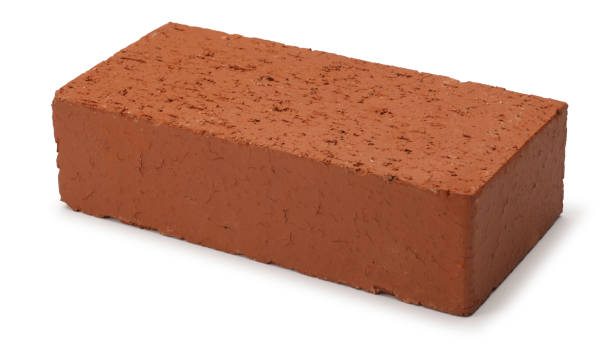
\includegraphics[height=1in]{Silde_Template/images/brick.jpeg}
%   \end{column}
%   \begin{column}{0.33\textwidth}
%   \centering
%     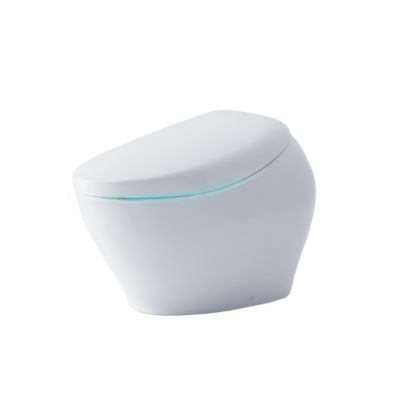
\includegraphics[height=1in]{Silde_Template/images/toilet.jpeg}
%   \end{column}
%     \begin{column}{0.33\textwidth}
%     \centering
%     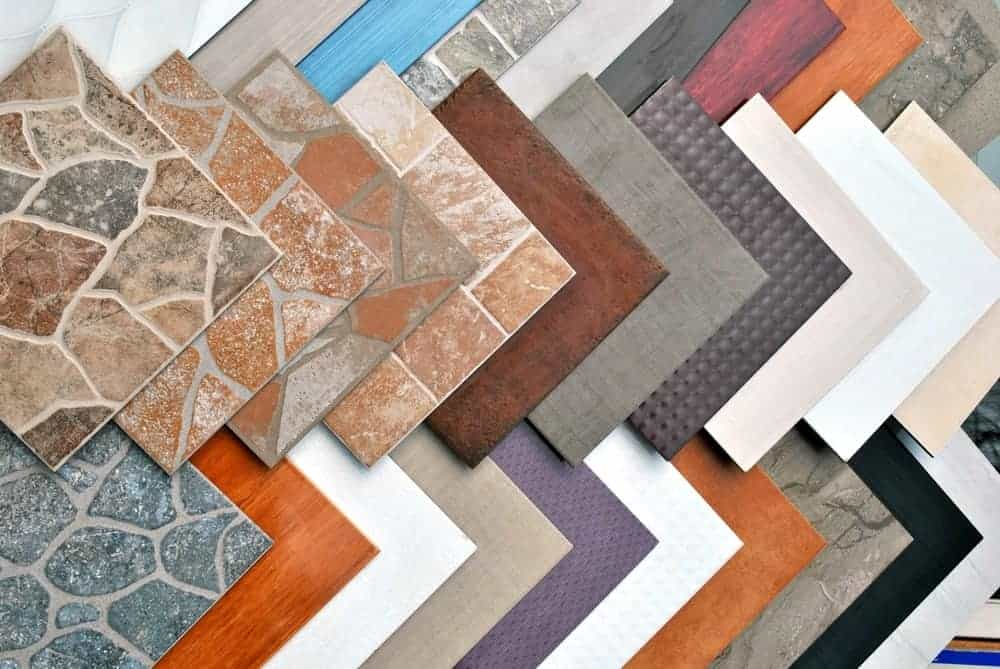
\includegraphics[height=1in]{Silde_Template/images/tiles.jpeg}
%   \end{column}
% \end{columns}
% \pause
% \begin{itemize}
%     \item Generally based on clay or silica
%     \item can require complex processing or tooling
% \end{itemize}
% \end{frame}

% \begin{frame}{Advanced or Technical Ceramics}

% \textbf{Advanced Ceramics}
% Advanced ceramics are newer materials, such as laser host materials, piezoelectric ceramics, and ceramics
% for dynamic random access memories (DRAMs), among others, which are often produced in small quantities at higher prices.    
% \vspace{1em}

% \begin{columns}
%   \begin{column}{0.33\textwidth}
%     \centering
%     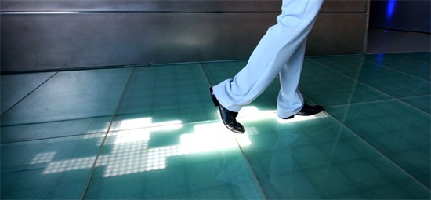
\includegraphics[height=1in]{Silde_Template/images/piezoelectric_floor.png}
%   \end{column}
%   \begin{column}{0.33\textwidth}
%     \centering
%     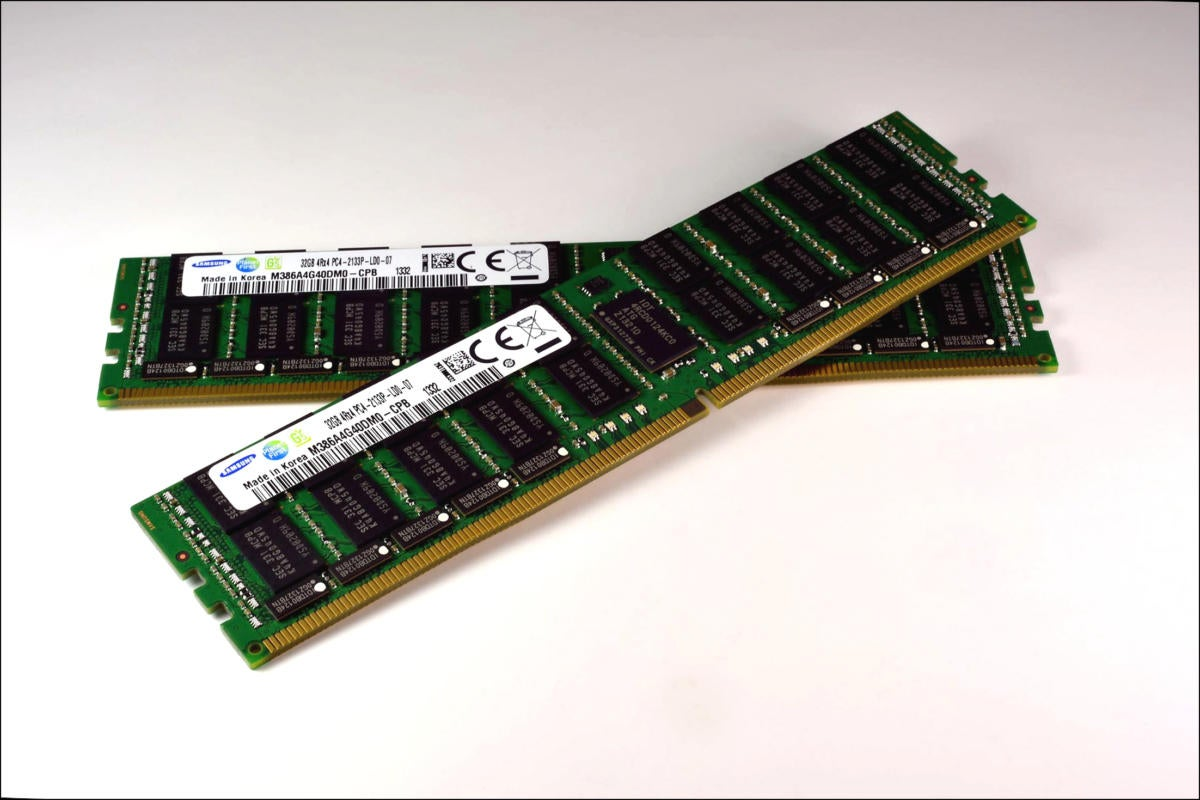
\includegraphics[height=1in]{Silde_Template/images/DRAM.jpeg}
%   \end{column}
%     \begin{column}{0.33\textwidth}
%     \centering
%     
\includegraphics[height=1in]{Silde_Template/images/ballistic ceramics.jpeg}
%   \end{column}
% \end{columns}
% \pause
% \vspace{1em}

% \begin{itemize}
%     \item They exhibit superior mechanical properties, corrosion/oxidation resistance, or electrical, optical and/or magnetic properties.
%     \item Emerged primarily over the last 100 years
% \end{itemize}

% \end{frame}

% \begin{frame}{Properties and Applications of Ceramics}
% \centering
% 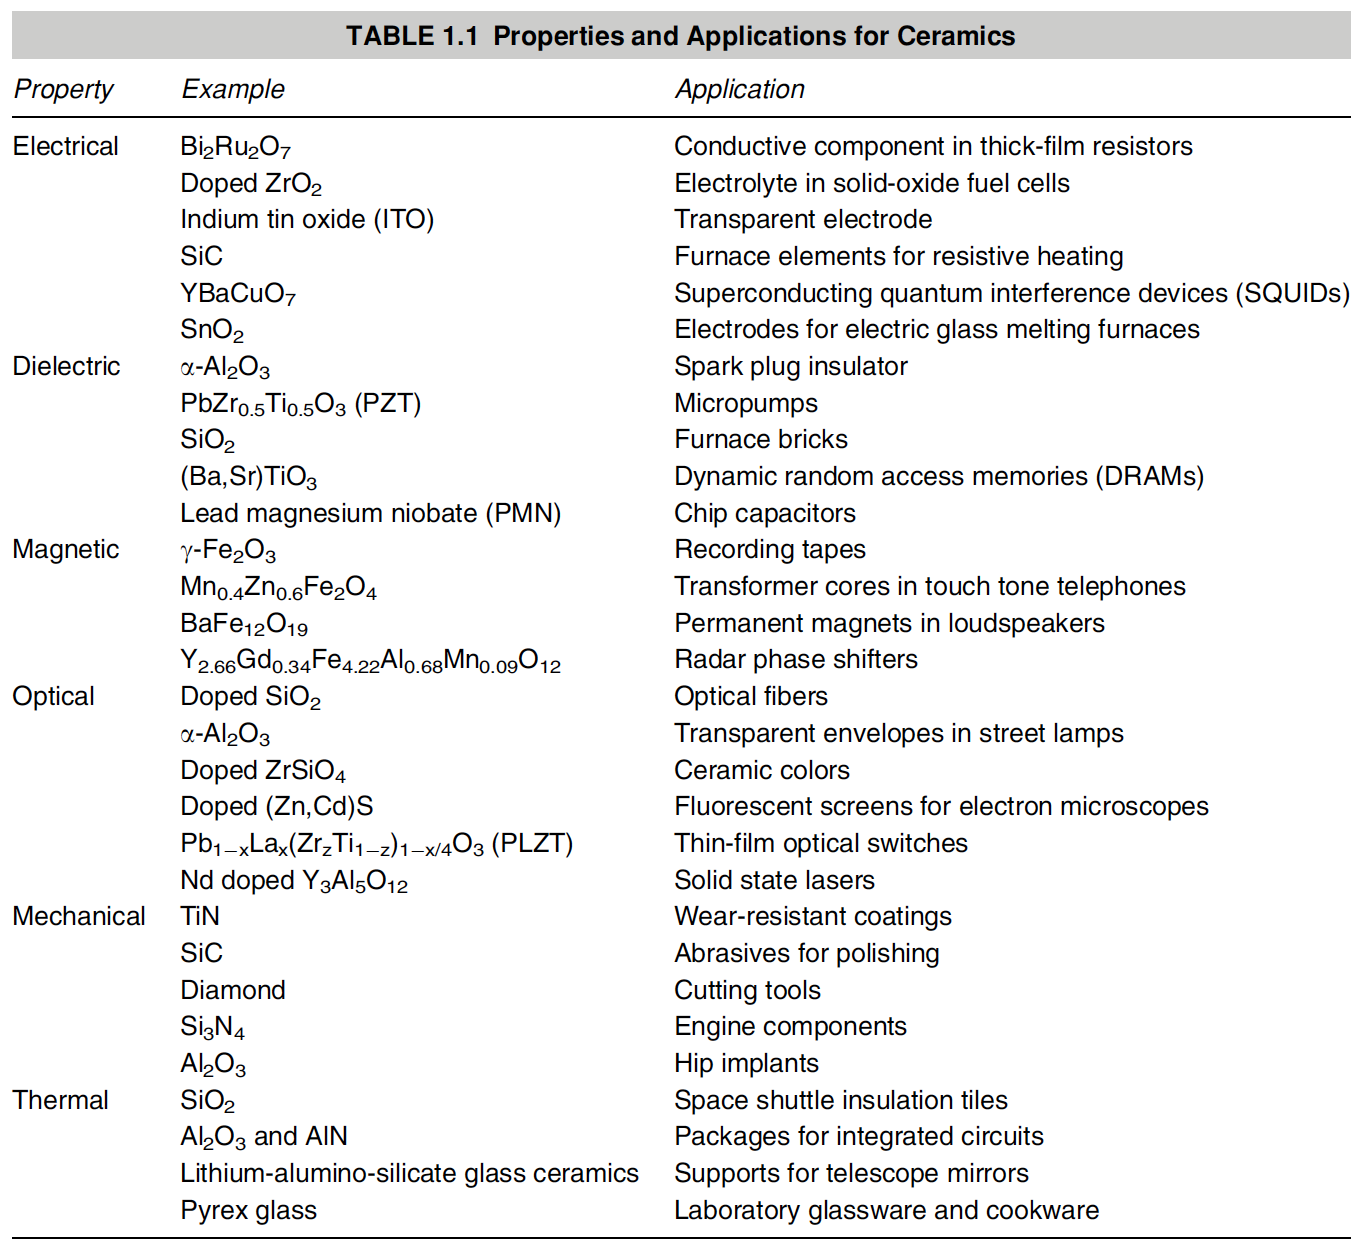
\includegraphics[height=\textheight]{Silde_Template/images/Properties of ceramics.png}
% \end{frame}

% \begin{frame}{Advanced vs. Traditional Ceramics}
% \centering
% 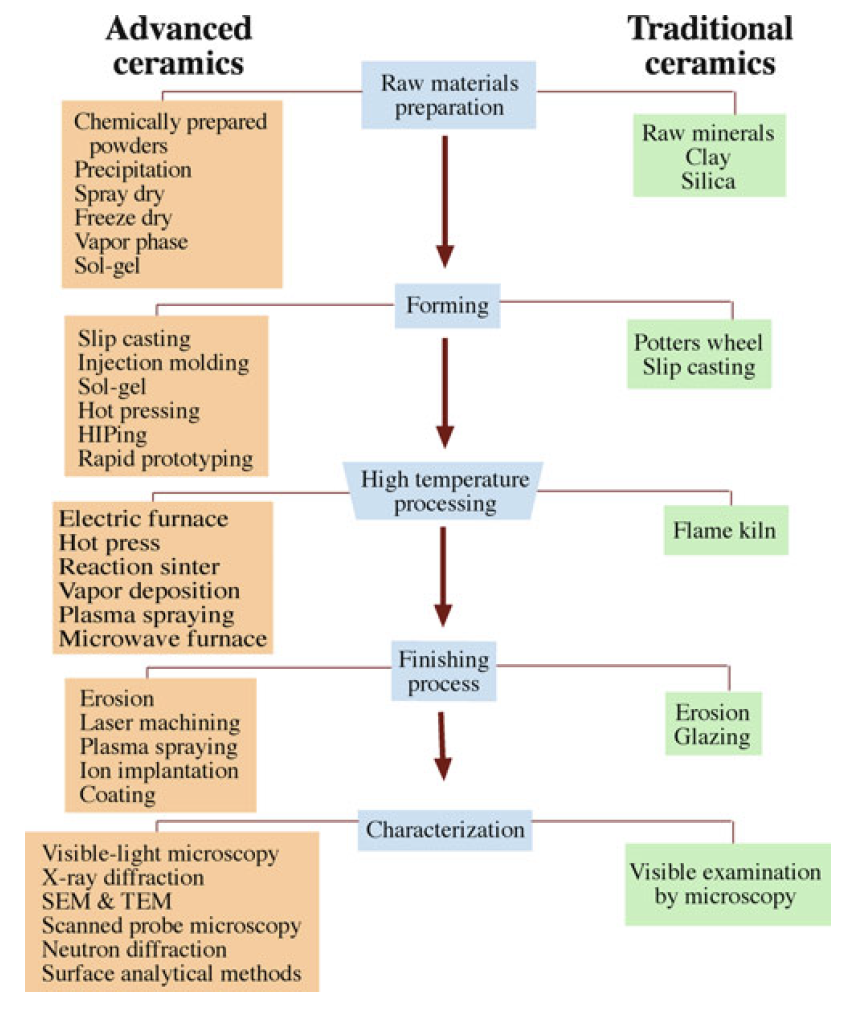
\includegraphics[height=\textheight]{Silde_Template/images/Comparison.png}
% \end{frame}

% \section{Market and Future}

% \begin{frame}{Overall Market Finances}
% Ceramics is a multibillion-dollar industry. Worldwide sales are about \$100 billion per year; the U.S. market alone is over \$35 billion annually.
% \vspace{1em}

% \centering
% 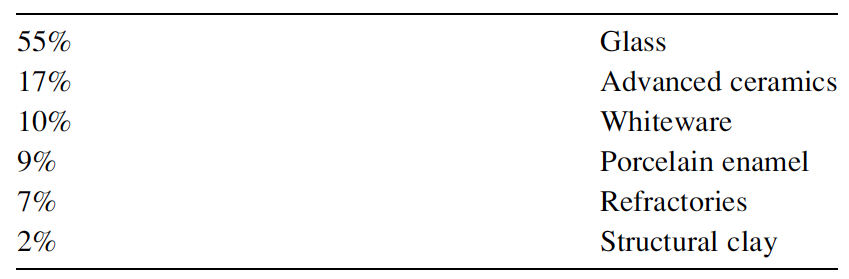
\includegraphics[width=0.75\textwidth]{Silde_Template/images/general market.png}
% \vspace{1em}

% \begin{itemize}
%     \item Bricks and glass, the commodity ceramics have the largest market
% \end{itemize}
    
% \end{frame}

% \begin{frame}{Advanced Ceramics}
% \vspace{1em}

% \centering
% 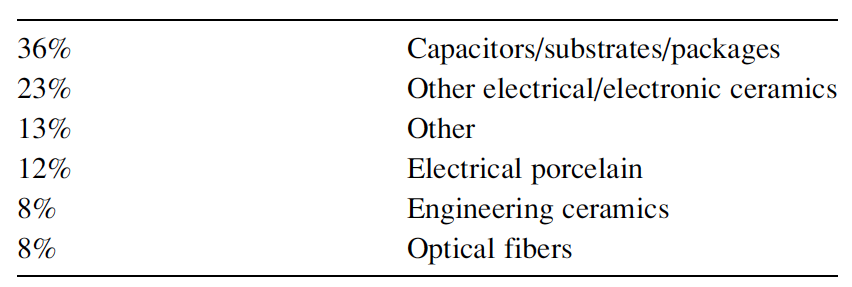
\includegraphics[width=0.6\textwidth]{Silde_Template/images/advanced ceramics.png}

% \begin{itemize}
%     \small
%     \item More than half of this sector is comprised of electrical and electronic ceramics and ceramic packages \pause
%     \item Significant growth areas include microwave filters and resonators for use in wireless communication \pause
%     \item Engineering ceramics, also called structural ceramics, include wear-resistant components such as dies, nozzles,and bearings\pause
%     \item Bioceramics (e.g., ceramic and glass-ceramic implants and dental crowns) account for about 20\% of this market (dental crowns) \pause 
%     \item Porcelain enamel is the ceramic coating applied to many steel appliances such as kitchen stoves, washers and dryers \pause
%     \item More than 50\% of refractories are consumed by the steel industry \pause
% \end{itemize}
% \end{frame}

% \begin{frame}{Structural Ceramics}
% \begin{itemize}
%     \item Include silicon nitride ($Si_3N_4$), silicon carbide ($SiC$), zirconia ($ZrO_2$), boron carbide ($B_4C$), and alumina ($Al_2O_3$)
%     \pause
%     \item They are used in applications such as cutting tools, wear components, heat exchangers, and engine parts
%     \pause
%     \item The relevant properties of structural ceramics are high hardness, low density, high-temperature mechanical strength, creep resistance, corrosion resistance, and chemical inertness
%     \pause
% \end{itemize}
% \vspace{1em}

% \textbf{Key Issues}
% \begin{itemize}
%     \item Reducing the cost of the final product
%     \item Improving reliability
%     \item Improving reproducibility
% \end{itemize}

% \end{frame}

% \begin{frame}{Electrical Ceramics}
% \begin{itemize}
%     \item Include barium titanate ($BaTiO_3$), zinc oxide ($ZnO$), lead zirconate titanate [$Pb(Zr_xTi_{1-x})O_3$], aluminum nitride ($AlN$), and high-temperature superconductors \pause
%     \item They are used in applications as diverse as capacitor dielectrics, varistors, micro-electro-mechanical systems (MEMS), substrates, and packages for integrated circuits \pause
% \end{itemize}

% \textbf{Key Issues}
% \begin{itemize}
%     \item Integrating with existing semiconductor technology
%     \item Improving processing
%     \item Enhancing compatibility with other materials
%     \item Improved electrical resistivity in thin films
% \end{itemize}

% \end{frame}

% \begin{frame}{Bioceramics}
% \begin{itemize}
%     \item The response of these materials varies from nearly inert to bioactive to resorbable \pause
%     \item Nearly inert bioceramics include alumina ($Al_2O_3$) and zirconia ($ZrO_2$) \pause
%     \item Bioactive ceramics include hydroxyapatite and some special glass and glass-ceramic formulations \pause
%     \item Tricalcium phosphate, which dissolves in the body, is an example of a resorbable bioceramic \pause
% \end{itemize}

% \textbf{Key Issues}
% \begin{itemize}
%     \item Matching mechanical properties to human tissues
%     \item Increasing reliability
%     \item Enhancing compatibility with other materials
%     \item Improving processing methods
% \end{itemize}
    
% \end{frame}

% \begin{frame}{Coating and Films}
%     \begin{itemize}
%         \item Coatings and films are generally used to modify the surface properties of a material (e.g., a bioactive coating deposited on the surface of a bio-inert implant) \pause
%         \item They may also be used for economic reasons: we may want to apply a coating of an expensive material on a lower cost substrate rather than make the component entirely from the more expensive material \pause $\rightarrow$ An example is applying a diamond coating on a cutting tool \pause
%         \item Thin film properties can be better, the transport properties of thin films of HTSCs, which are improved over the bulk
%     \end{itemize}


% \textbf{Key Issues}
% \begin{itemize}
%     \item Understanding film deposition and growth
%     \item Improving film/substrate adhesion
%     \item Increasing reproducibility
% \end{itemize}

% \end{frame}
% \begin{itemize}
%     \item Composites may use ceramics as the matrix phase and/or the reinforcing phase \pause
%     \item The purpose of a composite is to display a combination of the preferred characteristics of each of the components \pause
%     \item Ceramic matrix composites increase fracture toughness through reinforcement with whiskers or fibers \pause
%     \item Metal matrix composites usually an increase in strength, enhanced creep resistance, and greater wear resistance \pause
% \end{itemize}
% \begin{frame}{Composites}

% \textbf{Key Issues}
% \begin{itemize}
%     \item Reducing processing costs
%     \item Developing compatible combinations of materials (e.g., matching coefficients of thermal expansion)
%     \item Understanding interfaces
% \end{itemize}

% \end{frame}

% \begin{frame}{Nanoceramics}
% \begin{itemize}
%     \item Widely used in cosmetic products (e.g., sunscreens), as stabilizers, and they are critical in many catalytic applications \pause
%     \item Modern applications in quantum dots, fuel cells, and specialty coating applications \pause
% \end{itemize}

% \textbf{Key Issues}
% \begin{itemize}
%     \item Making them
%     \item Integrating them into devices through either top-down or bottom-up approaches
%     \item Ensuring that they do not have a negative impact on society
% \end{itemize}

% \end{frame}

\end{document}



        
